% ........................................................................... %

We give here some background knowledge on timed automata, a model that has been extensively used in the field of real-time model checking, and that will be useful for the remainder of this work. We begin with an overview of the model before focusing on the common problems (e.g., closure under complementation and reachability analysis). We then review some classes of timed automata that are interesting for this work, before finishing with model checking tools. \\

This will turn out to be useful later in the remainder of this work. Indeed, our approach for analyzing services business protocols completely depends on the closure under intersection and complementation in timed automata. It  also depends on the ability to perform location reachability analysis using a model checking tool.

% ........................................................................... %

\section{Overview}

% ........................................................................... %

We start with an overview of the model of timed automata, including its semantics. We then turn our attention to the ``classic'' problems such as closure under intersection or language inclusion.

% ........................................................................... %

\subsection{Model and semantics}

% ........................................................................... %

Timed automata were introduced in \cite{RADLD94} as an extension of classical automata \cite{Hopcroft79} to model real-time systems. Some preliminary works appeared in \cite{RACC94}. We start by an informal example before going through the formalization and semantics of the model.

\begin{figure}[htbp]
    \centering
    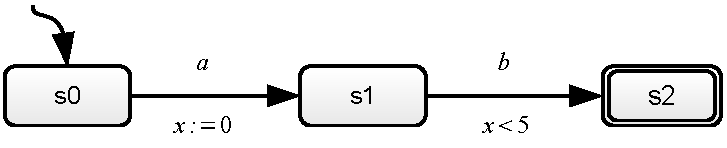
\includegraphics[width=0.9\textwidth]{content/timed-automata/sample-ta}
    \caption{A sample timed automaton $A$.}
    \label{fig:sample-ta}
\end{figure}

\paragraph{Extension of automata with clocks.}
We take as an example the timed automaton $A$ depicted on Figure~\ref{fig:sample-ta}. At first sight, $A$ is much like a ``normal'' automaton: it has locations (e.g., $s_0, s_1$ and $s_2$) as well as switches with labels over the alphabet $\Sigma = \{ a, b \}$. There is one initial location $s_0$ while $s_2$ is an accepting location. Hence, an (untimed) word $a \cdot b$ can be recognized by $A$ while words such as $a \cdot a$ or $b \cdot a$ cannot. Timing constraints are added in $A$ by making use of a clock $x$ which is a continuous variable over the set of real-valued numbers $\Rpos$. Of course, a timed automaton can have more than one clock. $A$ recognizes the set of timed words $a \cdot b$ such that $b$ is recognized at most 5 units of time after $a$. To do that, the clock $x$ is reset to $0$ when the automaton switches from the location $s_0$ to $s_1$ on the symbol $a$. Again, a switch can reset an arbitrary number of clocks. Initially, every clock is set to $0$ and then, they grow synchronously as time evolves. Clocks can be used in constraints attached to the switches, called guards, and that can enable or disable a switch depending on how those boolean functions over the clocks evaluate. Here, the clock $x$ is used in the guard of the $b$-labeled switch so that $b$ cannot be recognized when $(x \geq 5)$ is true.\\

Time elapses in the locations, while the switches are instantaneous. It is also possible to bound the time spent in the locations by defining clocks constraints called \emph{invariants}, which can be used to force switches to be fired before the invariants conditions become violated. Indeed, it is a requirement that time can always elapse in the locations. Timed automata recognize \emph{timed words} which are sequences in which a non-negative real value is attached to each symbol. For example $w = (a, 0) \cdot (b, 1)$ is a timed word where $b$ has been recognized 1 unit of time after $a$. More precisely, a timed word over an alphabet $\Sigma$ is a sequence $(a_0,t_0) \cdot (a_1, t_1) \cdots (a_n, t_n)$ such that $a_i \in \Sigma$,  $t_i \in \Rpos$ and  $t_0 < t_1 < \cdots < t_n$.

\paragraph{Clocks valuations.}
In what follows, we reuse the same notations as in \cite{RADLD94,RA98}.
Given a set of clocks $X$ with their values being in $\Rpos$, a clocks valuation $v$ for $X$ is a function $X \longrightarrow \Rpos$ that associates to each clock $x \in X$ its value $v(x)$. The set of clocks valuations for $X$ is written $\Rpos^X$. The set of clocks constraints over $X$ is $\mathcal{C}(X)$, built using boolean combinations of atomic constraints of the form $x \;\#\; c$ with $x \in X$, $\;\#\; \in \{=, \neq, <, \leq, >, \geq \}$ and $c \in \Q$. $\mathcal{C}_{\prec}(X)$ is the restrictions of $\mathcal{C}(X)$ where the clocks constraints are of the form $x < c$ or $x \leq c$. A clocks valuation $v$ satisfies an atomic constraint $(x \;\#\; c)$ if and only if $(v(x) \;\#\; c)$ is true. This allows to check whether a complete constraint $g$ can be satisfied by a clocks valuation $v$, denoted as $v \models g$. Given $d \in \Rpos$, $v' = v + d$ is the clocks valuation such that $v'(x) = v(x) + d$ for each $x \in X$. Also, given a subset of clocks $r \in X$, $v' = [r \leftarrow 0]v$ is the clocks valuation such that $v'(x) = 0$ if $x \in r$ and $v'(x) = v(x)$ if $x \in X \setminus \{ r \}$.

\begin{definition}[Timed automata] \cite{RADLD94,RA98}
  
A timed automaton $A$ is a tuple $A = (\Sigma, L, L^0, L^f, X, I, E)$ where:
\begin{itemize}

    \item $\Sigma$ is the \emph{alphabet},

    \item $L$ is a finite set of \emph{locations} (or states),

    \item $L^0 \subseteq L$ is the set of \emph{initial locations},

    \item $L^f \subseteq L$ is the set of \emph{final locations} (or accepting states),

    \item $X$ is a finite set of clocks,

    \item $I : L \rightarrow \mathcal{C}_{\prec}(X)$ associates an \emph{invariant} to each location

    \item $E \subseteq L \times \mathcal{C}(X) \times \Sigma \times 2^X \times L$ is a finite set of switches (or switches) $e = (l, g, a, r, l') \in E$ from $l$ to $l'$, where $g$ is the guard, $r$ is the set of clocks to be reset and $a$ is the label.

\end{itemize}
\end{definition}

A timed automaton $A$ recognizes timed words that are sequences of the form $(a_1, t_1) \cdot (a_2, t_2) \cdots (a_n, t_n)$ where given $i \in \{1, 2, \cdots, n\}$, $a_i \in \Sigma$ is a symbol from the alphabet and $t_i \in \Rpos$ is the time at which $a_i$ is recognized by $A$. The set of timed words recognized by a timed automaton $A$ is the timed language denoted as $L(A)$.

\paragraph{Semantics.}
The semantic of a timed automaton $A$ is defined using an (infinite) timed \emph{labeled transitions system} (LTS). Each state of the LTS is a pair $(l, v) \in L \times \Rpos^X$, called a \emph{configuration}, where $l$ is the current location in $A$ and $v$ is a clocks valuation. There are two types of transitions: \emph{action transitions} (labeled with a symbol of $\Sigma$) and \emph{time transitions} (labeled with a real-valued duration). More precisely, the semantic of $A = (L, L^0, L^f, X, I, E, \Sigma)$ is given by the LTS $\mathcal{S}_A = (S, s_0, \rightarrow, \Sigma)$ where:

\begin{itemize}

    \item $S = L \times \Rpos^X$,

    \item $s_0 = (l_0, v_0)$ with $l_0 \in L^0$ and $v_0(x) = 0$ $\forall x \in X$,

    \item $\rightarrow$ is the transition relation:
    \begin{itemize}

        \item action transitions: $(l, v) \stackrel{a}{\longrightarrow} (l', v')$ if and only if there exists
        $e = (l, g, a, r, l') \in E$ such that $v \models g$, $v' = [r \leftarrow 0]v$ and $v' \models I(l')$

        \item time transitions: if $d \in \Rpos$ then $(l, v) \stackrel{d}{\longrightarrow} (l, v + d)$ if and only if $v + d \models I(l)$.

    \end{itemize}

\end{itemize}

The LTS $\mathcal{S}_A$ starts from an initial state made from an initial location and each clock set to $0$. Then, either instantaneous action transitions occur (possibly resetting some clocks), or time transitions allow the clocks to grow synchronously. The executions over $\mathcal{S}_A$ match the timed words that can be recognized by $A$ when they start from the initial state of $\mathcal{S}_A$ and they can reach a final state.\\

\begin{figure}[htbp]
    \centering
    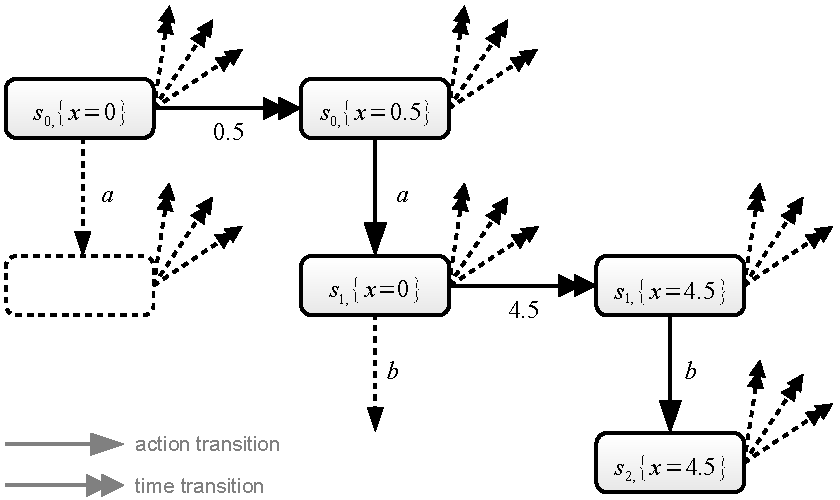
\includegraphics[width=\textwidth]{content/timed-automata/semantic-lts}
    \caption{The LTS $\mathcal{S}_A$ associated to the timed automaton $A$ of Figure~\ref{fig:sample-ta}.}
    \label{fig:semantic-lts}
\end{figure}

Let us consider again $A$ defined on Figure~\ref{fig:sample-ta} and its semantic LTS $\mathcal{S}_A$ which is depicted on Figure~\ref{fig:semantic-lts}. $(s_0, 0) \stackrel{1}{\longrightarrow} (s_0, 1) \stackrel{0.25}{\longrightarrow} (s_0, 1.25) \stackrel{a}{\longrightarrow} (s_1, 0) \stackrel{0.1}{\longrightarrow} (s_1, 0.1) \stackrel{b}{\longrightarrow} (s_2, 0.1)$ is a valid execution over $\mathcal{S}_A$ which recognizes the timed word $(a, 1.25) \cdot (b, 1.35)$ of the timed language $L(A)$.

% ........................................................................... %

\subsection{Classic problems}

% ........................................................................... %

We now review some classic problems for timed automata. They are summarized in Table~\ref{tab:ta-common-problems}.

\begin{table}[htbp]
\centering
\begin{tabular}{|p{7cm}|p{5cm}|}

    \hline

    \textit{Problem} &
    \textit{Results} \\

    \hline \hline

		Union & Closed \\ \hline
		
		Intersection & Closed \\ \hline
		
		Projection & Closed \\ \hline
		
		Complementation & Not closed \\ \hline
		
		Language inclusion & Undecidable \\ \hline
		
		Language equivalence & Undecidable \\ \hline
		
		Universality & Undecidable \\ \hline
		
		Language emptiness / reachability analysis & \textsc{PSPACE-Complete} \\ \hline

\end{tabular}
\caption{Classic problems for (general) timed automata \cite{RADLD94}.}
\label{tab:ta-common-problems}
\end{table}

\paragraph{Closure properties.}
Closure of timed automata under the following operators has been studied in \cite{RADLD94}: union, intersection, complementation and projection\footnote{Projection allows to map a timed language from one to another with a different alphabet (symbols that are not mapped are replaced by $\varepsilon$).}. Union and intersection are based on extensions of the classical procedures on automata \cite{Hopcroft79}. The closure under union and intersection is relatively easy. Closure under union comes from the fact that timed automata are indeterministic and support more than one location. Intersection is similar. The problematic non-closure under complementation is a consequence of indeterminism, as a timed word may have more than one execution. The proof is based on the observation that a timed word can have an execution ending in a final location and one in a non-final location, making it impossible to construct the complement like for untimed automata.

\paragraph{Timed language inclusion, equivalence and universality.}
We briefly introduce these three decision problems.
%
Given two timed automata $A$ and $A'$, the \emph{timed language inclusion problem} refers to checking if $\mathcal{L}(A) \subset \mathcal{L}(A')$. Similarly, the \emph{timed language equivalence problem} refers to checking if $\mathcal{L}(A) = \mathcal{L}(A')$. Finally, the \emph{universality problem} refers to checking whether a timed automaton $A$ defined over an alphabet $\Sigma$ is able to recognize all of the possible timed words over $\Sigma$.
%
These problems require the ability to complement timed automata. As an example, checking whether $\mathcal{L}(A) \subset \mathcal{L}(A')$ reduces to checking for the timed language emptiness of the automaton $A' \cap \overline{A}$. Unfortunately, timed automata are not closed under complementation, making these problems undecidable.
%
Checking for the emptiness of a timed language is a \textsc{PSPACE-Complete} problem. This problem is also referred to as the \emph{location reachability} problem (i.e., a timed language is empty if no final location can be reached.

\begin{figure}[htbp]
    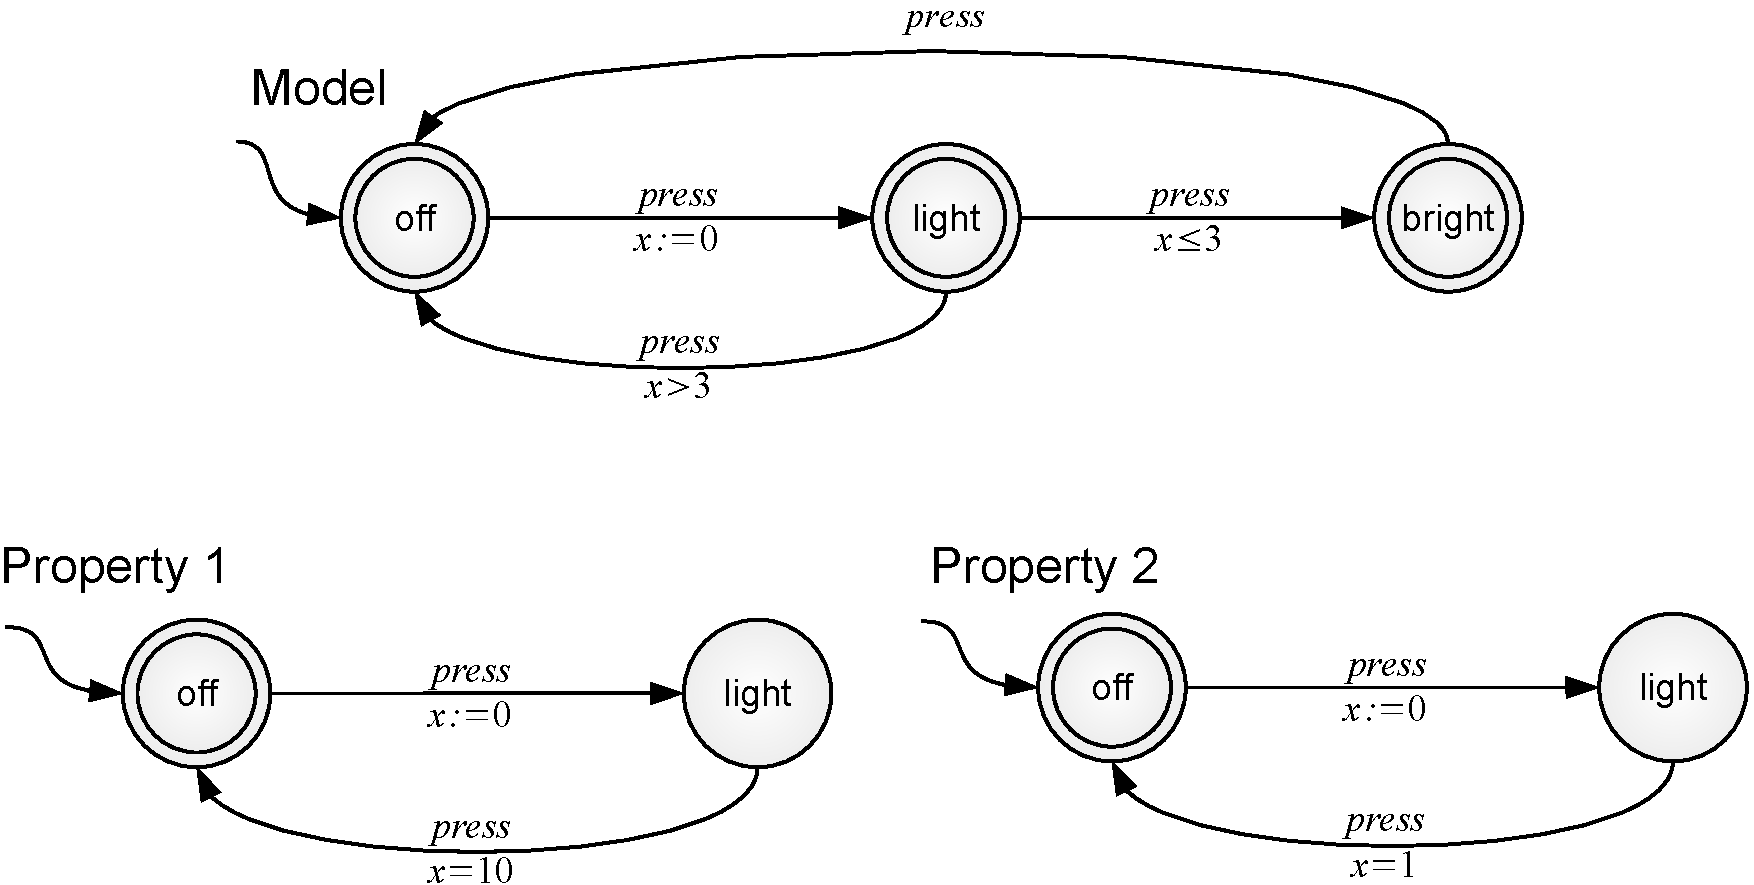
\includegraphics[width=\textwidth]{content/timed-automata/light-verification-inclusion}
    (\textit{model from} \url{http://www.cis.upenn.edu/~alur/Talks/sfm-rt-04.ppt})
    \caption{A model checking example that reduces to state reachability analysis.}
    \label{fig:light-verification-inclusion}
\end{figure}

\paragraph{Verification through test automata.}
In this case, the property to verify is expressed as a timed automaton, referred to as a \emph{test timed automaton}. The verification is performed by a reduction to a reachability / emptiness analysis. We give an example on Figure~\ref{fig:light-verification-inclusion}. The system that is modeled is a light controller. The light is initially turned off, and pressing it will turn it on. However, if the button is pressed twice quickly (within at most 3 units of time), then the light will be brighter. Finally, pressing the button another time will turn the light off.

We express two properties on this system using timed automata. The first one (property one) is used to test whether pressing the button once, then 10 units of time later will turn it off again. This is property that we expect to be satisfied by the modeled system. In turn, we do not expect the second property to be true: when pressed quickly twice, the light should not be turned off.

Model-checking through the mean of test automata is not always the best option, as verification reduces to a timed language inclusion checking problem. While checking for timed language emptiness is decidable (yet \textsc{PSPACE-Complete}), the non-closure under complementation is problematic. We will see later in this chapter that some classes of timed automata do not suffer from this issue. Back to the example of Figure~\ref{fig:light-verification-inclusion}, this is possible as the automata are deterministic.

% ........................................................................... %

\section{Classes of timed automata}

% ........................................................................... %

Several classes and extensions of timed automata have been studied. Indeed, the fact that the decision problems seen above are undecidable in the general case motivated such research directions. We summarize here the principal classes and extensions of timed automata that turned out to be useful in the context of this work.
%
Table~\ref{tab:ta-classes-decidability} summarizes the results regarding the timed language inclusion and emptiness checking problems, while Table~\ref{tab:ta-classes-expressiveness} details the results on expressiveness.
%
Further pointers can be found in \cite{RAPM04,RA98,ST03,JOJW04,BL-VAT06}.

\begin{table}[htbp]
\centering
\footnotesize
\begin{tabular}{|p{5cm}|p{4.5cm}|p{2.5cm}|}

	\hline
	
	\textit{Class or extension} &
	\textit{Emptiness checking} &
	\textit{Language inclusion} \\
	
	\hline \hline
	
	  Timed automata &
    \textsc{PSPACE-Complete} &
    Undecidable \\

    \hline

    Deterministic timed automata &
    \textsc{PSPACE-Complete} &
    Decidable \\

    \hline

    Event-clock automata &
    \textsc{PSPACE-Complete} &
    Decidable \\

    \hline

    Robust timed automata &
    \textsc{PSPACE-Complete} &
    Undecidable \\

    \hline \hline

    $\varepsilon$-transitions without clocks resets &
    \textsc{PSPACE-Complete} &
    Undecidable \\

    \hline

    $\varepsilon$-transitions with clocks resets &
    \textsc{PSPACE-Complete} &
    Undecidable \\

    \hline

    Diagonal constraints ($x - y \;\#\; c$)&
    \textsc{PSPACE-Complete} &
    Undecidable \\

    \hline

    Additive constraints ($x + y \;\#\; c$) &
    Decidable for 1 or 2 clocks, open problem for 3 clocks and undecidable starting from 4 clocks \cite{BerDuf-IPL2000} &
    Undecidable \\

    \hline
    
    Constraints of the form $x = 2y$ &
    Undecidable \cite{RADLD94} &
    Undecidable \\
    
    \hline
    
    Constraints with irrational constants &
    Undecidable \cite{Miller00} &
    Undecidable \\

    \hline

    Non-standard ($x := 0$) clocks resets &
    Decidable for $x := c$, undecidable for $x := x -1$ and decidable for $x := x + 1$ if diagonal constraints are not allowed \cite{BDFP04} &
    Undecidable \\
    
    \hline

\end{tabular}
\caption{Emptiness and timed language inclusion checking results for some classes and extensions of timed automata.}
\label{tab:ta-classes-decidability}
\end{table}

\begin{table}[htbp]
\centering
\footnotesize
\begin{tabular}{|p{5cm}|p{7.5cm}|}

    \hline

    \textit{Class or extension} &
    \textit{Observations} \\

    \hline \hline

    Deterministic timed automata &
    Strictly less expressive than timed automata \\

    \hline

    Event-clock automata &
    Indeterministic event-clock automata can always be rendered deterministic while this is not the case for (general) timed automata \cite{RALF94} \\

    \hline

    Robust timed automata &
    Robust timed languages are \emph{open} and their expressiveness is not comparable with the one of timed languages \cite{RAPM04} \\

    \hline \hline

    $\varepsilon$-transitions without clocks resets &
    The silent transitions can be removed \cite{VDPG97} \\

    \hline

    $\varepsilon$-transitions with clocks resets &
    Strictly more expressive than general timed automata: the silent transitions that reset clocks cannot be removed in general \cite{VDPG97,BBVD+99,LSV:07:12} \\

    \hline

    Diagonal constraints ($x - y \;\#\; c$)&
    More concise than timed automata, but not more expressive \cite{BBVD+99} \\

    \hline

    Additive constraints ($x + y \;\#\; c$) &
    More expressive than timed automata \\

    \hline

\end{tabular}
\caption{Expressiveness of some classes and extensions of timed automata.}
\label{tab:ta-classes-expressiveness}
\end{table}

\paragraph{Deterministic timed automata.}
The class of \emph{deterministic timed automata} has been defined in \cite{RADLD94}. It restricts the definition of timed automata by:
\begin{enumerate}
  
  \item allowing only a single initial location, and
  
  \item requiring that given two switches from the same source location having the same input symbol, their guards are disjoint so as to preserve determinism.
  
\end{enumerate}
As such, the timed automaton of Figure~\ref{fig:sample-ta} is deterministic. This is also true for the timed automata depicted on Figure~\ref{fig:light-verification-inclusion}.
Each timed word that is recognized by a deterministic timed automaton has exactly one accepting run over it. Deterministic timed automata form a strict subclass of timed automata (they are less expressive). The problem of the determinization of indeterministic (untimed) automata is decidable \cite{Hopcroft79}. This is however not the case for timed automata \cite{ST03}.

\paragraph{Event-recording timed automata.}
Event-clock automata, and more particularly \emph{event-recording automata} form an interesting class of timed automata \cite{RALF94}. In this model, clocks are assigned to the input symbols. Each time one of symbol is recognized (e.g., $a$), its associated clock is reset (e.g., $x_a$). The time domain $\T$ is the set of positive reals $\Rpos$ augmented with the $\perp$ symbol to denote the fact that a given symbol has not been recognized yet (i.e., every clock is set to $\perp$ initially). The fundamental property in event-recording automata is that the value of clocks only depends on the input word. The consequence of this is that such automata are \emph{determinizable} (i.e., an indeterministic event-recording automaton can always be transformed into a deterministic one that recognizes the same language) and \emph{complementable} (i.e., event-recording automata are closed under complementation). Extensions of event-recording automata can be defined as long as the value of clocks only depends on the input word.

\paragraph{Silent transitions.}
In the case of untimed automata, they do not add to the expressiveness and they can be removed easily \cite{Hopcroft79}. This is however not the case with timed automata, and as we will see later in this thesis, this will be a major issue for the decidability of timed protocol operators, as the model of timed protocols exhibits such transitions. Indeed, allowing silent ($\varepsilon$) transitions in timed automata strictly adds to the expressiveness \cite{VDPG97,BBVD+99,LSV:07:12}. Complex techniques exist to remove the $\varepsilon$-transitions when they do not reset clocks \cite{VDPG97}. However, this is not possible in the general case when they do reset clocks, i.e., there exist switches of the form $l \xrightarrow{\varepsilon, g, \{ x \}} l'$. Of special interest is the notion of \emph{precise actions} defined in \cite{BBVD+99}, as it gives a tool for proving that some timed languages cannot be recognized by a timed automaton without $\varepsilon$-labeled switches. We will leverage this tool when studying the expressiveness of timed protocols.

\paragraph{Other classes.}
Some classes or extensions have different expressiveness levels compared to (general) timed automata. The expressiveness of the class of \emph{Robust timed automata}\footnote{Briefly, a robust timed automaton recognizes  timed words with some fuzziness in the event dates as no real world system can be expected to be as precise as timed automata expectations.} cannot be compared to the one of timed automata \cite{RAPM04}. The classical decidability problems (reachability / emptiness, inclusion) remain unchanged.

The closure and decidability results remain unchanged compared to (general) timed automata in the following cases: constraints of the form $x = 2y$, constraints with irrational constants, and allowing non-standard (i.e., $x := 0$) clocks resets.

In most cases, the emptiness / reachability problem is decidable (yet \textsc{PSPACE-Complete}) despite the language inclusion problem being undecidable because of non-closure under complementation. However, some forms of modified clocks constraints and clocks resets can render it undecidable \cite{BerDuf-IPL2000,RADLD94,Miller00,BDFP04,BBVD+99,LSV:07:12,VDPG97}.

\paragraph{Other formalisms.}
Several formalisms have been introduce to capture timing constraints. Among them, a common abstraction is to define delays with minimum and maximum values on timed transition systems: \cite{HenzingerMP94,MerrittMT91,LynchA92,PnueliH88}.

Petri nets support extensions with timing requirements \cite{petrinets}. \emph{Timed Petri nets} are an extension where a transition can be fired only if its enabling duration is in a certain time window \cite{PMM74}. In turn, \emph{Timed Petri nets} associate to each transition a set of time windows \cite{Ramchandani74}. The tokens that circulate in timed Petri nets are given an age. A transition can then be fired only by tokens whose ages are in one of the time windows of the transition.

Lots of contributions bridging timed automata and timed Petri nets have been made. The work done in \cite{BHR-ICALP2006} is of most interest as it proves that timed Petri nets are not more expressive than timed automata with respect to the language equivalence. It introduces a class called \emph{Read-arc timed Petri nets} which is language-equivalent to timed automata.

\paragraph{Temporal logics.}
They have been traditionally used for formal verification purposes. A temporal logic formula  expresses some form of \emph{qualitative time} property such as \emph{``when the light is off, pressing the button will turn it on''}. To put it another way, temporal logics allow to specify the order of events. However, it is not possible to express \emph{quantitative time} properties such as \emph{``when the light is off and the button is pressed twice in less than 2 seconds, the light will be bright''}.

The purpose of a temporal logic formula is to check wether there exists a path to a state that satisfies the formula in the considered system. Two branches of temporal logics exist:
\begin{enumerate}
  
  \item \emph{linear-time temporal logics} allow reasoning over a single time line, and
  
  \item \emph{branching-time temporal logics} allow reasoning over several time lines.
  
\end{enumerate}
CTL, which stands for \emph{computational tree logic}, is the traditional branching-time logic \cite{ClarkeES86} while LTL (\emph{linear temporal logic}) is the traditional linear-time logic \cite{Pnueli77}.

Both CTL and LTL have been extended to support quantitative time. TCTL (\emph{timed computational tree logic}) \cite{HNSY94} extends the branching-time logic CTL. Similarly, MTL (\emph{metric temporal logic}) \cite{Koymans90} and TPTL (\emph{timed propositional temporal logic}) \cite{AlurH89,AlurH94} extend the linear-time temporal logic LTL to support quantitative time. Some fragments of MTL have been defined to seek better decidability results: as MITL (\emph{metric interval logic}) \cite{AlurFH96}, Safety-MTL \cite{OuaknineW05} and coFlat-MTL \cite{BouyerMOW07}. 

\begin{table}[htbp]
\centering
\footnotesize
\begin{tabular}{|p{3.5cm}|p{9cm}|}

    \hline

    \textit{Logic} &
    \textit{Model-checking problem} \\
    
    \hline
    
    TCTL &
    \textsc{PSPACE-Complete} \cite{AlurCD90,AlurCD93} \\
    
    \hline
    
    \multirow{2}{5cm}{MTL over finite runs} &
    Decidable and non-primitive recursive under the pointwise semantics \cite{OW07} \\
    
    \cline{2--2} &
    Undecidable under the continuous semantics \cite{AlurFH96} \\
    
    \hline
    
    MTL over infinite runs &
    Undecidable under pointwise semantics \cite{OuaknineW06} \\
    
    \hline
    
    TPTL over finite runs &
    Undecidable under the pointwise and continuous semantics \cite{AlurH94} \\
    
    \hline
    
    MITL over infinite runs &
    \textsc{EXPSPACE-Complete} \cite{AlurFH96} \\
    
    \hline
    
    Safety-MTL over infinite runs &
    Decidable but not primitive-recursive under the pointwise semantics \cite{OuaknineW05} \\
    
    \hline
    
    coFlat-MTL over infinite runs &
    \textsc{EXPSPACE-Complete} under the pointwise semantics \cite{BouyerMOW07} \\
    
    \hline
    

\end{tabular}
\caption{Results on the problem of model-checking using timed temporal logics.}
\label{tab:temporal-logics-checking}
\end{table}

The results on the problem of model-checking using timed temporal logics are summarized in Table~\ref{tab:temporal-logics-checking}. The branching-time logic TCTL offers very good decision problem properties while the linear timed temporal logics are much harder, if not decidable. The research on linear logics has been motivated by the fact that they are sometimes more powerful than the branching ones. A detailed survey on timed temporal logics can be found in \cite{Bouyer-M4M5}.

% ........................................................................... %

\section{Software tools}

% ........................................................................... %

\begin{figure}[htbp]
    \centering
    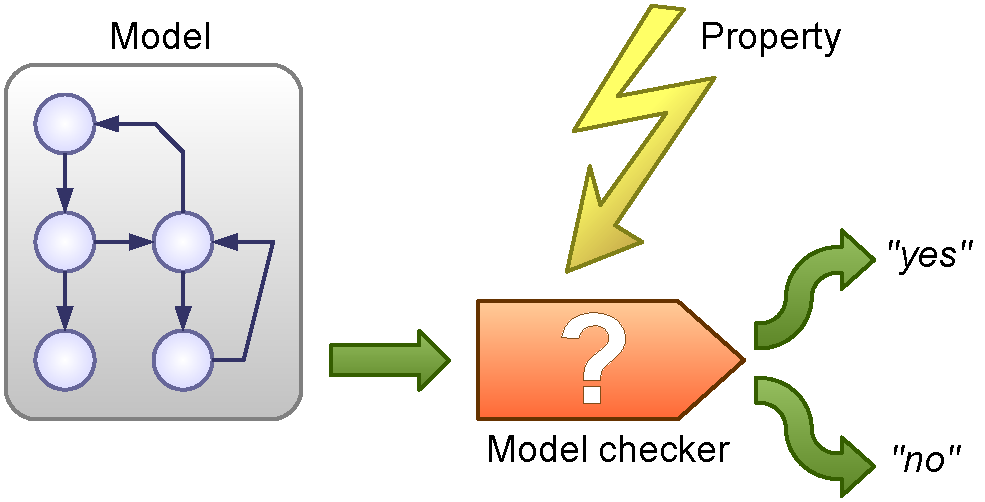
\includegraphics[width=0.9\textwidth]{content/timed-automata/model-checking}
    \caption{Principle of model checking.}
    \label{fig:model-checking}
\end{figure}

We briefly introduce the general principle of \emph{model checking} that we illustrated on Figure~\ref{fig:model-checking}. It refers to the process of testing \emph{properties} of a system for which a \emph{model} is given. The \emph{model checker} is a ``black box'' component that takes both of them as inputs then outputs whether the property is satisfied or not. Some model checkers can also output a \emph{trace}, mostly to give details of why the property cannot be satisfied (they are sometimes referred as \emph{error traces}).\\

The types of properties to be checked are usually classified in the following categories, although a model checker does not especially distinguish them. \emph{Reachability properties} check whether a property can possibly be satisfied by the system (e.g., \emph{``the light can be switched off''}). \emph{Safety properties} state that something which is considered as ``bad'' will never happen in the system (e.g., \emph{``the light cannot stay on for more than 20 minutes''}). Finally, \emph{liveness properties} state that something which is considered as ``good'' will eventually happen (e.g., \emph{``when the light is off, pressing the button turns it on''}).\\

Various timed automata model checkers have been proposed. They target different classes of timed automata as a model. They leverage timed temporal logics for expressing properties and query the models. We briefly present the main tools.\\

\begin{table}[htbp]
\footnotesize
\centering
\begin{tabular}{|p{4cm}|p{4cm}|p{4cm}|}

	\hline

	\textit{Tool} &
	\textit{Model} &
	\textit{Temporal logic} \\
	
	\hline
	
	Kronos \cite{KRONOS1,KRONOS2} &
	Timed automata &
	TCTL \\
	
	\hline
	
	HyTech \cite{HYTECH} &
	Hybrid automata \cite{ACHH93,alur97symbolic}  &
	ICTL, an extension of TCTL \cite{ACHH93} \\
	
	\hline
	
	UPPAAL \cite{UPPAAL} &
	Hybrid extension of timed automata &
	Subset of TCTL \\
	
	\hline
	
	Tempo \cite{MS01} &
	Event-recording timed automata &
	\emph{Event-recording fixpoint logic} defined in \cite{MS01} \\
	
	\hline

\end{tabular}
\label{tab:ta-model-checkers}
\caption{Model checking tools for classes and extensions of timed automata.}
\end{table}

\begin{figure}[htbp]
    \centering
    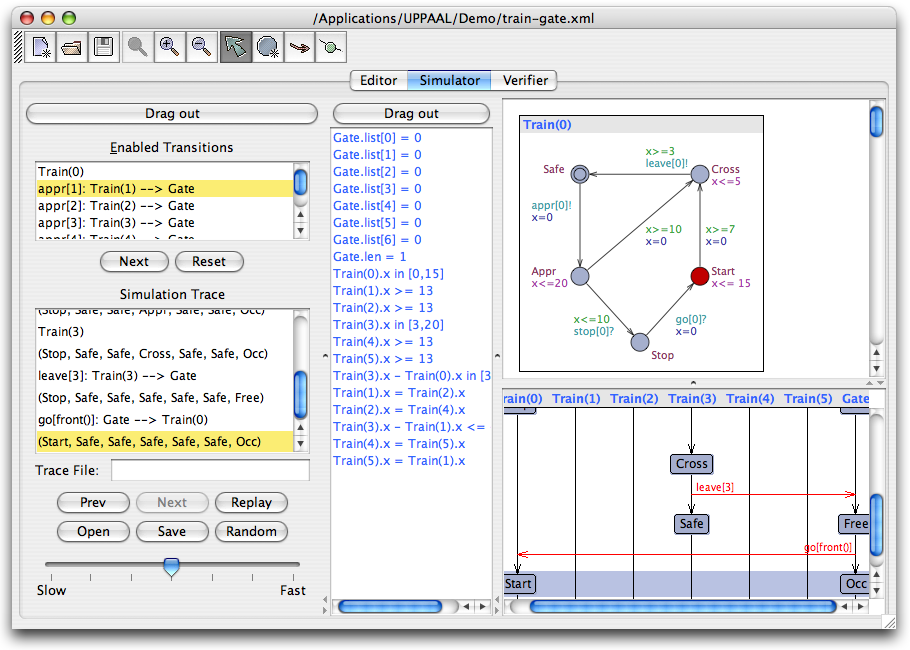
\includegraphics[width=\textwidth]{content/timed-automata/uppaal-2}
    \caption{A screenshot of UPPAAL.}
    \label{fig:uppaal}
\end{figure}

The tools are presented in Table~\ref{tab:ta-model-checkers}. Not surprisingly, branching timed temporal logics are popular given the decidability of the model checking problem. Tempo is specialized on event-recording timed automata and uses a logic developed on purpose. Kronos is the only tool to use ``canonical'' timed automata while UPPAAL and HyTech both use hybrid extensions. Briefly, an hybrid system \cite{alur97symbolic} features both continuous (e.g., variables in $\R$) and discrete behavior (e.g., variables in $\N$). At the time of the writing of this document, it should be noted that UPPAAL is the only actively developed project. UPPAAL has also managed to emerge from an academic research prototype to a commercial product for model checking. It has been used in several industrial studies (a complete list is available at \url{http://www.it.uu.se/research/group/darts/uppaal/examples.shtml}). We give a few references containing such case studies: \cite{HSLL97, HLS99, DAKRT97, LAAB98, dw00, lpw:tacas98, bowman98automatic, BGKLLPY96, lp:prfts97}.\\

A screenshot of the UPPAAL simulation environment is available on Figure~\ref{fig:uppaal}. A more detailed presentation of UPPAAL is available in the appendix from page~\pageref{chap:uppaal}.

% ........................................................................... %